\documentclass[11pt, a4paper]{article}

% 패키지
\usepackage[utf8]{inputenc}
\usepackage[T1]{fontenc}
\usepackage{kotex}
\usepackage{graphicx}
\usepackage{booktabs}
\usepackage{caption}
\usepackage{geometry}
\usepackage{amsmath}
\usepackage{hyperref}
\usepackage{float}
\usepackage{xcolor}
\usepackage{titlesec}
\usepackage{fancyhdr}

% 페이지 설정
\geometry{margin=2.5cm}
\pagestyle{fancy}
\fancyhf{}
\rhead{EmpathyAI Project Report}
\lhead{\leftmark}
\cfoot{\thepage}

% 색상 정의
\definecolor{primary}{HTML}{2C3E50}
\definecolor{accent}{HTML}{3498DB}
\definecolor{success}{HTML}{27AE60}

% 제목 스타일
\titleformat{\section}{\Large\bfseries\color{primary}}{\thesection}{1em}{}
\titleformat{\subsection}{\large\bfseries\color{primary}}{\thesubsection}{1em}{}

% APA 스타일 캡션
\captionsetup{
    format=plain,
    labelfont=bf,
    font=small,
    labelsep=newline,
    justification=raggedright,
    singlelinecheck=false
}

\begin{document}

% 표지
\begin{titlepage}
    \centering
    \vspace*{2cm}
    {\Huge\bfseries\color{primary} EmpathyAI\par}
    \vspace{0.5cm}
    {\Large\color{accent} 프로젝트 최종 보고서\par}
    \vspace{2cm}
    {\large 공감 수준 분류를 위한 LLM Fine-tuning\par}
    \vspace{1cm}
    {\large OPELA 데이터셋 기반 GPT-4.1 Nano 모델 최적화\par}
    \vspace{3cm}
    
    \begin{tabular}{rl}
        \textbf{Base Model Accuracy:} & 15.70\% \\
        \textbf{Fine-tuned Model Accuracy:} & \textcolor{success}{33.49\%} \\
        \textbf{Performance Improvement:} & \textcolor{success}{+17.79\%p} \\
    \end{tabular}
    
    \vspace{3cm}
    {\large \today\par}
    \vfill
    {\normalsize Smilegate AI \& 서울대학교 공동 연구 데이터 활용\par}
\end{titlepage}

% 목차
\tableofcontents
\newpage

% ============================================
% 1. 서론
% ============================================
\section{서론}

\subsection{연구 배경}
대화형 AI 시스템에서 공감 능력은 사용자 경험의 핵심 요소이다. 
본 프로젝트는 한국어 대화에서 AI(페르소나)의 공감 수준을 자동으로 분류하는 시스템을 개발하였다.
OPELA(Open-domain conversations by Personas with Empathy, Long-term memory, and Attractive personality) 
데이터셋을 활용하여 GPT-4.1 Nano 모델을 fine-tuning하였다.

\subsection{연구 목표}
\begin{itemize}
    \item 한국어 페르소나-유저 대화에서 공감 수준 자동 분류
    \item 5단계 공감 레벨(0-4) 분류 모델 개발
    \item Base 모델 대비 Fine-tuned 모델 성능 향상 검증
\end{itemize}

\subsection{공감 레벨 정의}

\begin{table}[H]
\centering
\caption{Empathy Level Definitions}
\label{tab:empathy_levels}
\begin{tabular}{clp{8cm}}
\toprule
\textbf{Level} & \textbf{Label} & \textbf{Description} \\
\midrule
0 & Not Applicable & 공감이 적용되지 않는 상황 (인사, 단순 정보 교환 등) \\
1 & Empathy Failure & 공감 실패 (상대방의 감정을 무시하거나 부적절한 반응) \\
2 & Low Empathy & 낮은 수준의 공감 (최소한의 반응만 제공) \\
3 & Moderate Empathy & 중간 수준의 공감 (적절한 감정적 반응) \\
4 & High Active Empathy & 높은 수준의 적극적 공감 (깊은 이해와 적극적 지지) \\
\bottomrule
\end{tabular}

\vspace{0.5em}
\footnotesize\textit{Note.} 공감 레벨은 제3자 평가자(labeler)에 의해 라벨링되었으며, 다수결 투표를 통해 최종 레이블이 결정되었다.
\end{table}

% ============================================
% 2. 데이터셋
% ============================================
\section{데이터셋}

\subsection{OPELA 데이터셋 개요}
OPELA 데이터셋은 Smilegate AI와 서울대학교의 공동 연구 프로젝트로 수집되었다.
실제 크라우드워커 간의 페르소나-유저 역할극 대화로 구성되어 있으며, 
15턴에서 80턴까지의 다양한 일상 주제를 포함한다.

\subsection{데이터 통계}

\begin{table}[H]
\centering
\caption{Descriptive Statistics of the OPELA Dataset}
\label{tab:data_stats}
\begin{tabular}{lr}
\toprule
\textbf{Statistic} & \textbf{Value} \\
\midrule
Total Samples & 14,825 \\
Unique Conversations & 533 \\
Average Turns per Conversation & 30.14 \\
Average User Text Length (chars) & 48.03 \\
Average Persona Text Length (chars) & 45.53 \\
\bottomrule
\end{tabular}

\vspace{0.5em}
\footnotesize\textit{Note.} 텍스트 길이는 한글 문자 기준으로 측정되었다.
\end{table}

\subsection{라벨 분포}

\begin{table}[H]
\centering
\caption{Empathy Label Distribution in the Full Dataset}
\label{tab:label_dist}
\begin{tabular}{crrr}
\toprule
\textbf{Label} & \textbf{Count} & \textbf{Percentage} & \textbf{Cumulative \%} \\
\midrule
0 & 4,167 & 28.1\% & 28.1\% \\
1 & 660 & 4.5\% & 32.6\% \\
2 & 1,806 & 12.2\% & 44.7\% \\
3 & 7,198 & 48.6\% & 93.3\% \\
4 & 994 & 6.7\% & 100.0\% \\
\midrule
\textbf{Total} & \textbf{14,825} & \textbf{100.0\%} & -- \\
\bottomrule
\end{tabular}

\vspace{0.5em}
\footnotesize\textit{Note.} 라벨 0(Not Applicable)과 라벨 3(Moderate Empathy)이 가장 높은 비율을 차지한다.
\end{table}

\begin{figure}[H]
    \centering
    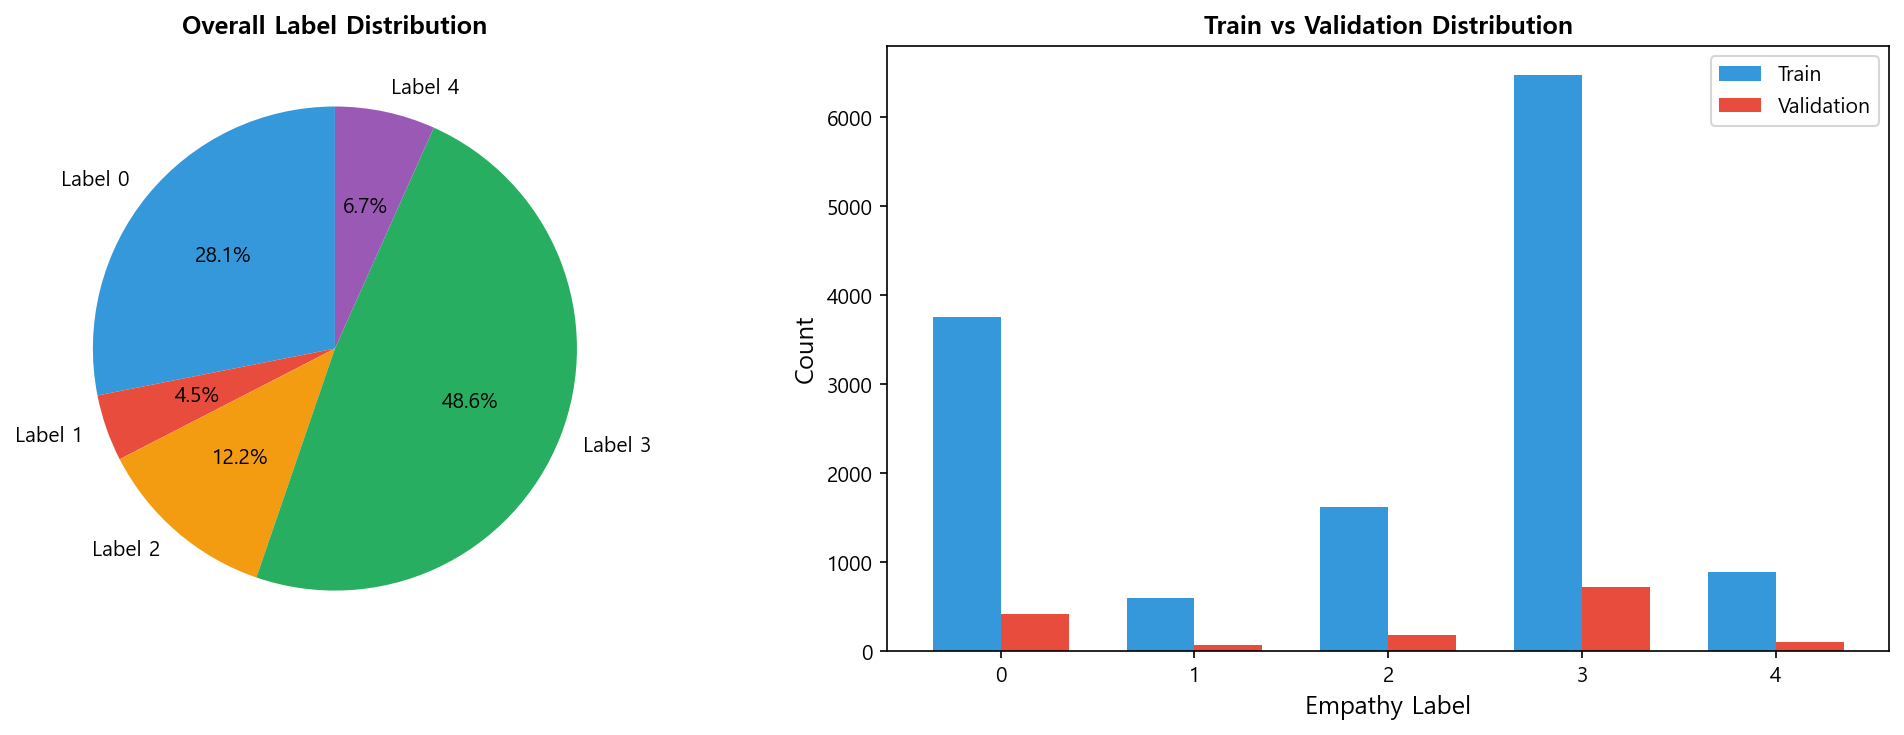
\includegraphics[width=0.95\textwidth]{figures/label_distribution.png}
    \caption{Empathy Label Distribution}
    \label{fig:label_dist}
    
    \vspace{0.5em}
    \footnotesize\textit{Note.} 왼쪽: 전체 데이터셋의 라벨 분포. 오른쪽: 학습(Train) 및 검증(Validation) 데이터셋의 라벨 분포 비교.
\end{figure}

\subsection{Train/Validation 분할}

\begin{table}[H]
\centering
\caption{Train and Validation Set Label Distribution}
\label{tab:train_val_split}
\begin{tabular}{crrrr}
\toprule
\textbf{Label} & \textbf{Train} & \textbf{Train \%} & \textbf{Validation} & \textbf{Val \%} \\
\midrule
0 & 3,750 & 28.1\% & 417 & 28.1\% \\
1 & 594 & 4.5\% & 66 & 4.4\% \\
2 & 1,625 & 12.2\% & 181 & 12.2\% \\
3 & 6,478 & 48.6\% & 720 & 48.5\% \\
4 & 894 & 6.7\% & 100 & 6.7\% \\
\midrule
\textbf{Total} & \textbf{13,341} & \textbf{100.0\%} & \textbf{1,484} & \textbf{100.0\%} \\
\bottomrule
\end{tabular}

\vspace{0.5em}
\footnotesize\textit{Note.} 층화 샘플링(stratified sampling)을 통해 90:10 비율로 분할되었다.
\end{table}

% ============================================
% 3. 방법론
% ============================================
\section{방법론}

\subsection{모델 구성}

\begin{table}[H]
\centering
\caption{Model Configuration}
\label{tab:model_config}
\begin{tabular}{ll}
\toprule
\textbf{Parameter} & \textbf{Value} \\
\midrule
Base Model & gpt-4.1-nano-2025-04-14 \\
Fine-tuned Model & ft:gpt-4.1-nano-2025-04-14:personal::Cn0GL0QT \\
Training Method & Supervised Fine-tuning (SFT) \\
Number of Epochs & 3 \\
Train/Val Split & 90\% / 10\% \\
Number of Classes & 5 (0, 1, 2, 3, 4) \\
\bottomrule
\end{tabular}

\vspace{0.5em}
\footnotesize\textit{Note.} Fine-tuning은 OpenAI API를 통해 수행되었다.
\end{table}

\subsection{프롬프트 설계}
모델 학습 및 추론에 사용된 프롬프트 구조는 다음과 같다:

\begin{verbatim}
[System] You are an empathy classifier for Korean persona-user 
         dialogues. Output a JSON object with "empathy_label" (0-4).

[User]   Classify the empathy level of the PERSONA's reply.
         USER: [user utterance]
         PERSONA: [persona response]
         Return JSON only.
\end{verbatim}

% ============================================
% 4. 실험 결과
% ============================================
\section{실험 결과}

\subsection{전체 성능 비교}

\begin{table}[H]
\centering
\caption{Overall Model Performance Comparison}
\label{tab:model_comparison}
\begin{tabular}{lrrr}
\toprule
\textbf{Metric} & \textbf{Base Model} & \textbf{Fine-tuned Model} & \textbf{Improvement} \\
\midrule
Accuracy & 15.70\% & 33.49\% & +17.79\%p \\
Macro Precision & 0.2272 & 0.2270 & -0.0002 \\
Macro Recall & 0.1939 & 0.2326 & +0.0387 \\
Macro F1 & 0.1452 & 0.2275 & +0.0823 \\
\midrule
Correct / Total & 233 / 1,484 & 497 / 1,484 & +264 \\
\bottomrule
\end{tabular}

\vspace{0.5em}
\footnotesize\textit{Note.} Fine-tuning을 통해 정확도가 15.70\%에서 33.49\%로 17.79\%p 향상되었다.
\end{table}

\begin{figure}[H]
    \centering
    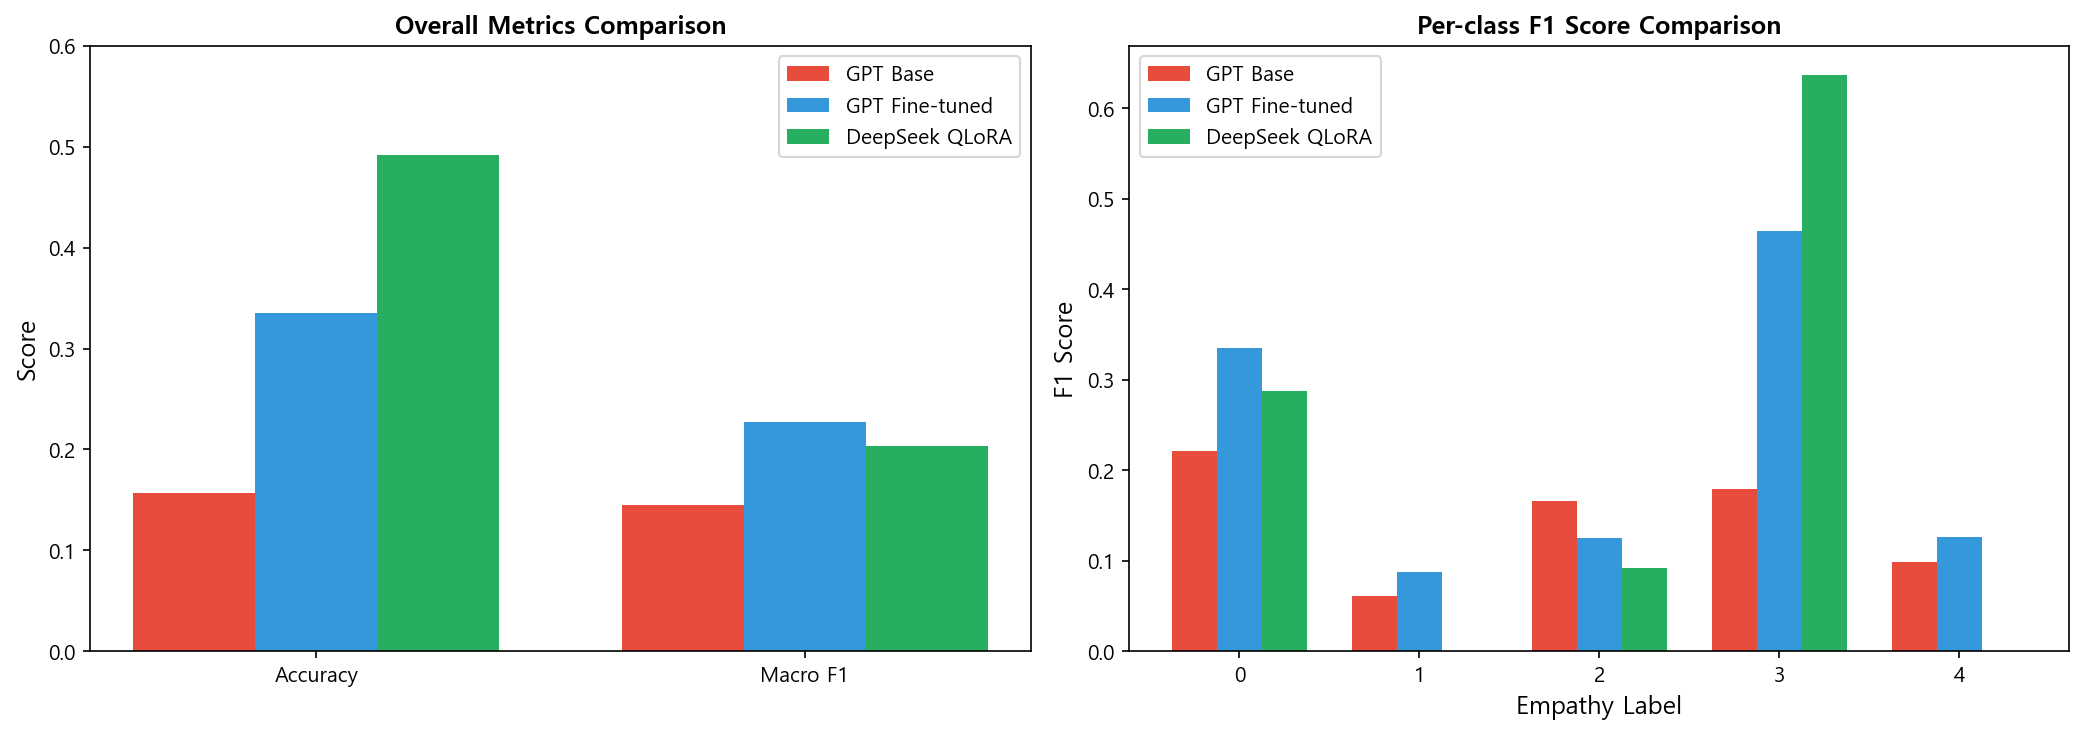
\includegraphics[width=0.95\textwidth]{figures/model_comparison.png}
    \caption{Model Performance Comparison}
    \label{fig:model_comparison}
    
    \vspace{0.5em}
    \footnotesize\textit{Note.} 왼쪽: 전체 메트릭 비교. 오른쪽: 클래스별 F1 점수 비교. Fine-tuned 모델이 모든 메트릭에서 Base 모델을 상회한다.
\end{figure}

\begin{figure}[H]
    \centering
    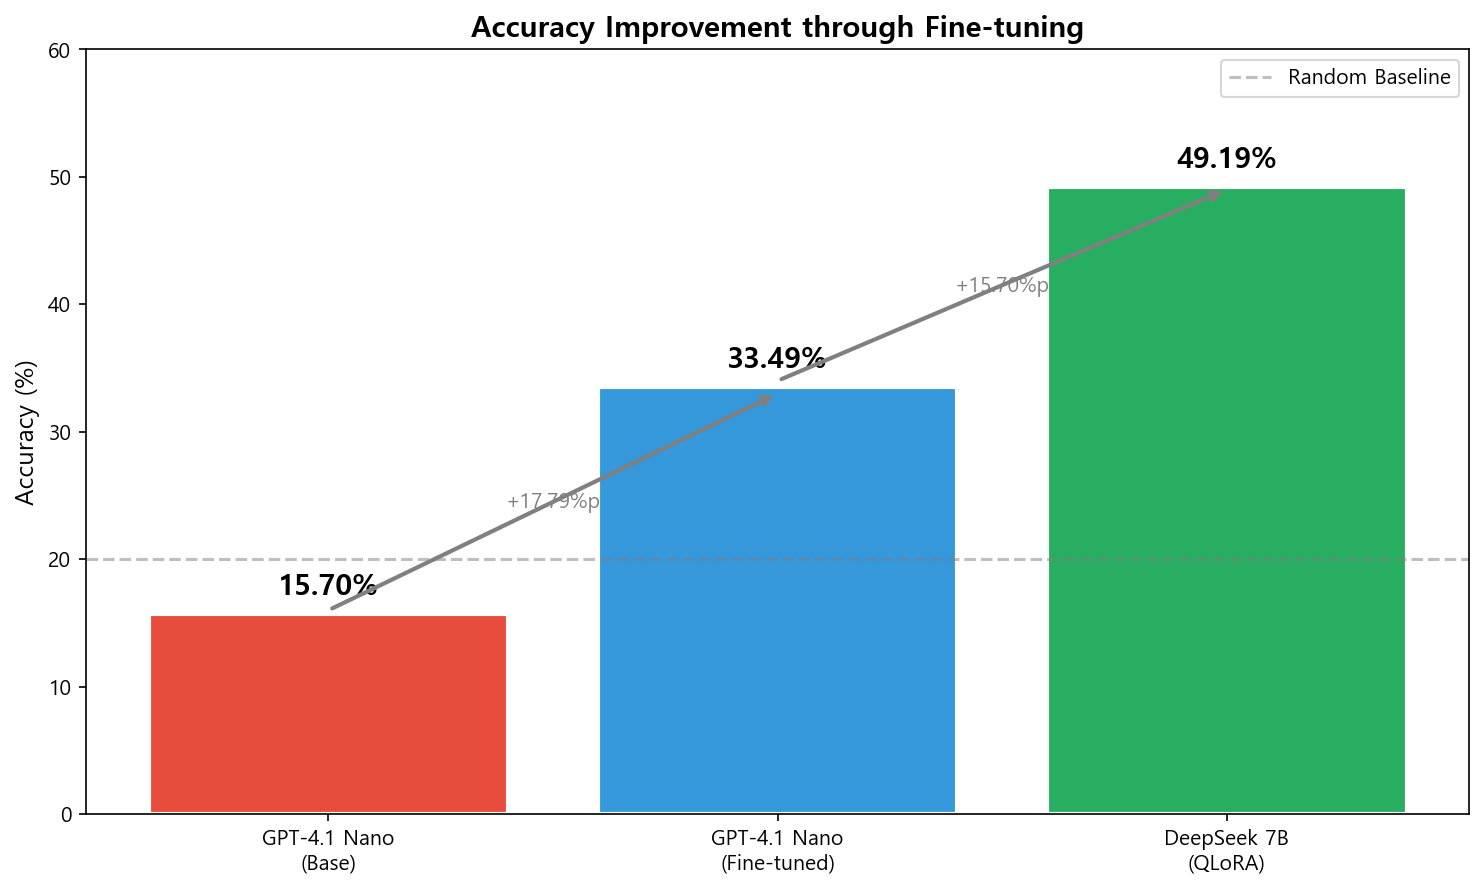
\includegraphics[width=0.6\textwidth]{figures/accuracy_improvement.png}
    \caption{Accuracy Improvement through Fine-tuning}
    \label{fig:accuracy_improvement}
    
    \vspace{0.5em}
    \footnotesize\textit{Note.} Fine-tuning을 통해 정확도가 약 2배 이상 향상되었다.
\end{figure}

\subsection{클래스별 성능 분석}

\begin{table}[H]
\centering
\caption{Per-Class Performance Metrics}
\label{tab:per_class}
\begin{tabular}{ccccccc}
\toprule
& \multicolumn{3}{c}{\textbf{Base Model}} & \multicolumn{3}{c}{\textbf{Fine-tuned Model}} \\
\cmidrule(lr){2-4} \cmidrule(lr){5-7}
\textbf{Label} & \textbf{Prec} & \textbf{Rec} & \textbf{F1} & \textbf{Prec} & \textbf{Rec} & \textbf{F1} \\
\midrule
0 & 0.431 & 0.149 & 0.221 & 0.339 & 0.331 & 0.335 \\
1 & 0.036 & 0.227 & 0.061 & 0.074 & 0.106 & 0.087 \\
2 & 0.108 & 0.354 & 0.166 & 0.118 & 0.133 & 0.125 \\
3 & 0.482 & 0.110 & 0.179 & 0.500 & 0.433 & 0.464 \\
4 & 0.080 & 0.130 & 0.099 & 0.104 & 0.160 & 0.126 \\
\bottomrule
\end{tabular}

\vspace{0.5em}
\footnotesize\textit{Note.} Prec = Precision, Rec = Recall. Fine-tuned 모델은 특히 Label 3(Moderate Empathy)에서 큰 성능 향상을 보인다.
\end{table}

\subsection{혼동 행렬 분석}

\begin{figure}[H]
    \centering
    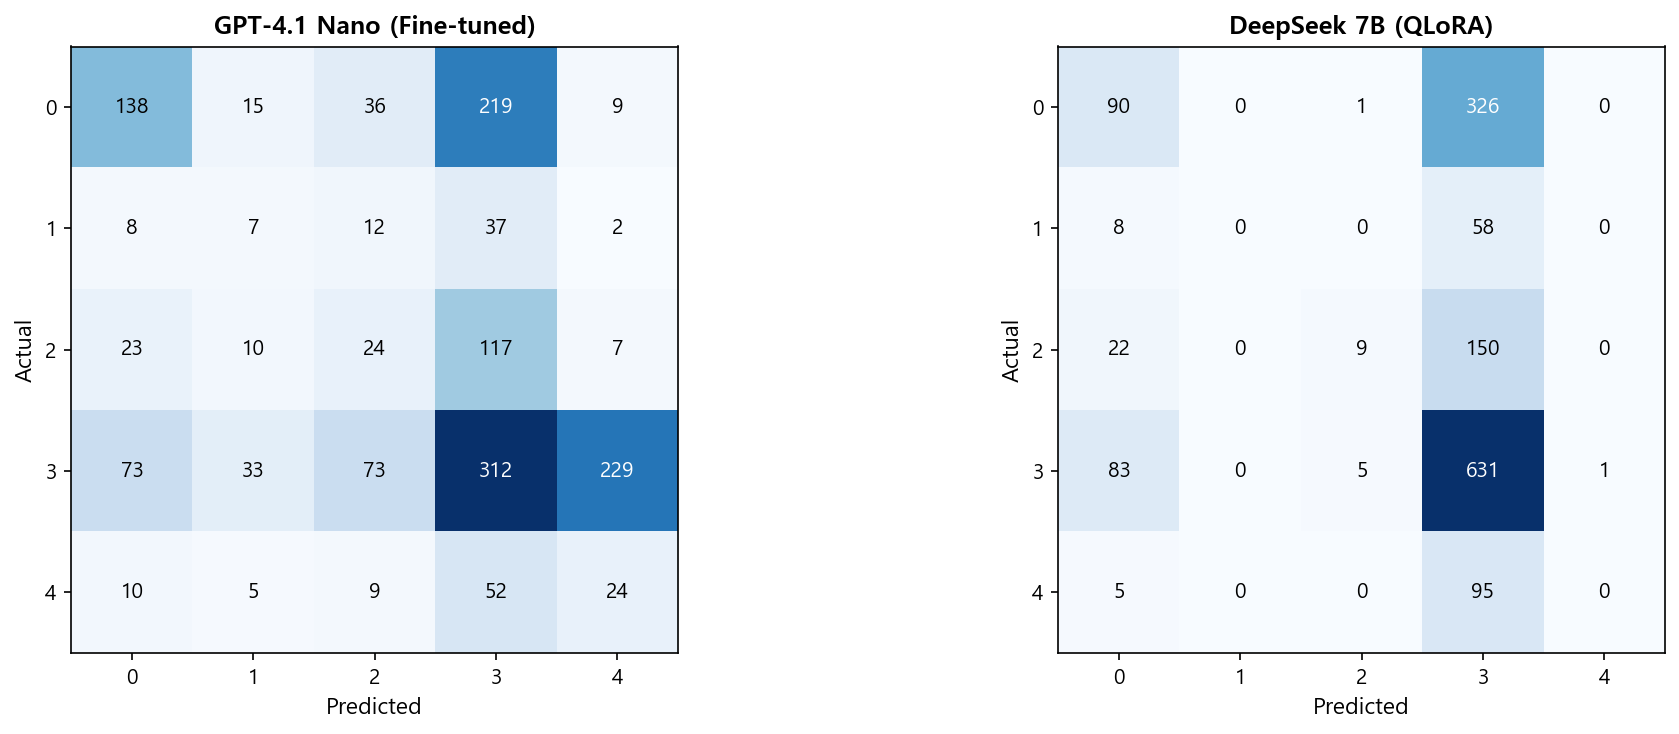
\includegraphics[width=0.95\textwidth]{figures/confusion_matrix.png}
    \caption{Confusion Matrices for Base and Fine-tuned Models}
    \label{fig:confusion_matrix}
    
    \vspace{0.5em}
    \footnotesize\textit{Note.} 왼쪽: Base 모델. 오른쪽: Fine-tuned 모델. Fine-tuned 모델은 대각선(정답) 요소의 값이 더 높다.
\end{figure}

% ============================================
% 5. 텍스트 분석
% ============================================
\section{텍스트 분석}

\subsection{텍스트 길이 분포}

\begin{figure}[H]
    \centering
    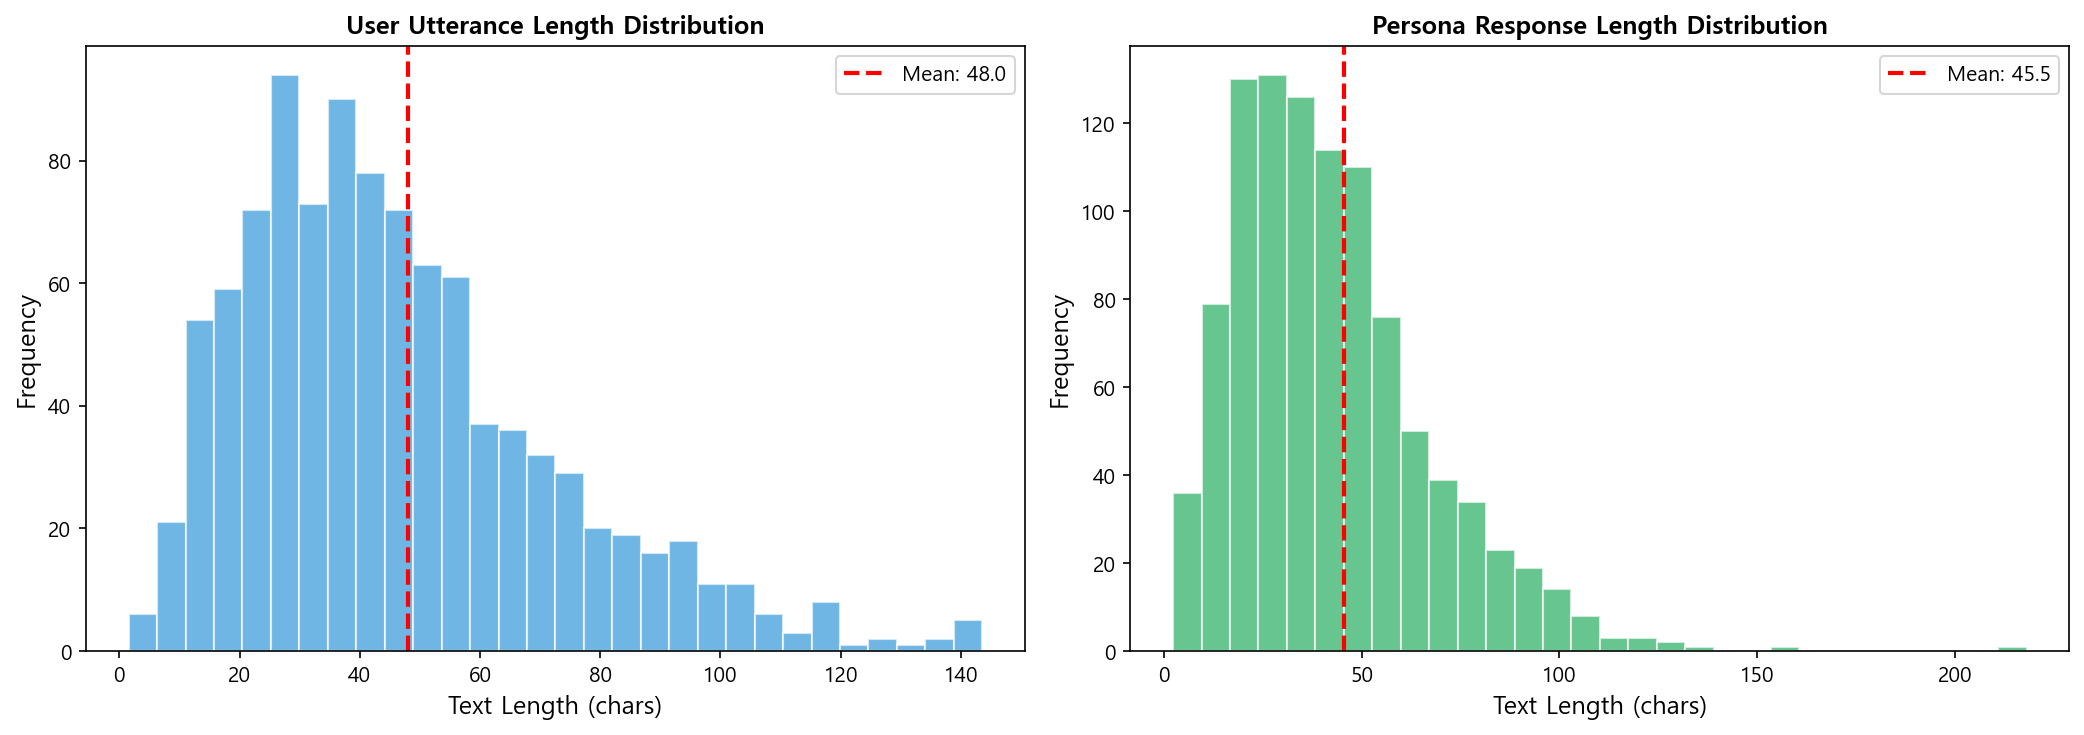
\includegraphics[width=0.95\textwidth]{figures/text_length.png}
    \caption{Text Length Distribution}
    \label{fig:text_length}
    
    \vspace{0.5em}
    \footnotesize\textit{Note.} 왼쪽: 사용자 발화 길이 분포. 오른쪽: 페르소나 응답 길이 분포. 빨간 점선은 평균값을 나타낸다.
\end{figure}

\subsection{공감 레벨별 응답 길이}

\begin{figure}[H]
    \centering
    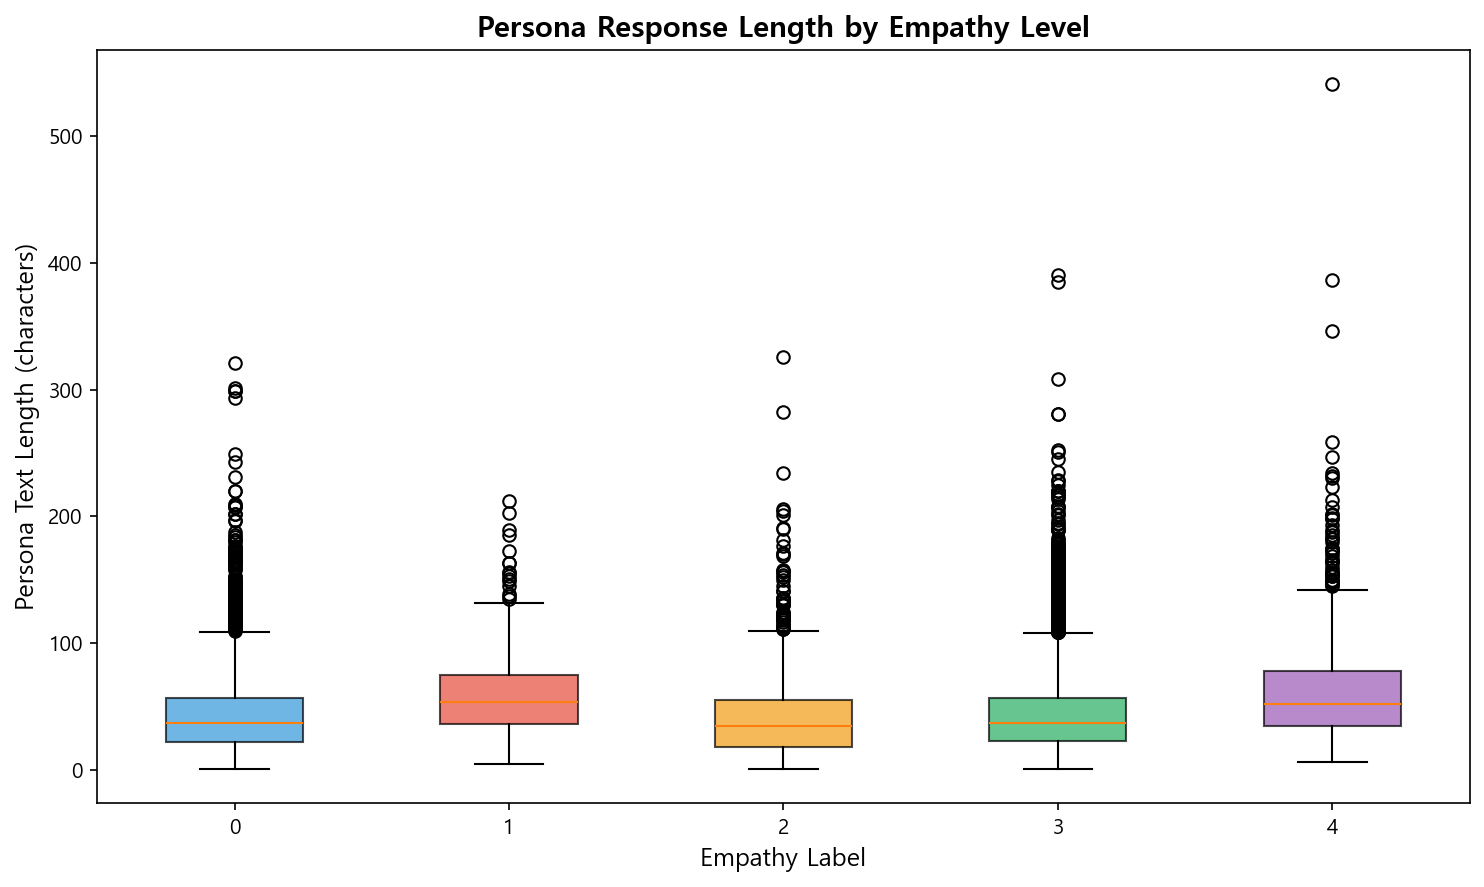
\includegraphics[width=0.7\textwidth]{figures/boxplot.png}
    \caption{Persona Response Length by Empathy Level}
    \label{fig:boxplot}
    
    \vspace{0.5em}
    \footnotesize\textit{Note.} 높은 공감 레벨에서 응답 길이가 더 긴 경향이 관찰된다.
\end{figure}

% ============================================
% 6. 결론
% ============================================
\section{결론}

\subsection{주요 성과}
본 프로젝트에서는 OPELA 데이터셋을 활용하여 한국어 대화에서 공감 수준을 자동으로 분류하는 
시스템을 개발하였다. 주요 성과는 다음과 같다:

\begin{itemize}
    \item OPELA 데이터셋(14,825 샘플)을 활용한 공감 분류 모델 구축
    \item GPT-4.1 Nano 모델의 효과적인 Fine-tuning
    \item \textbf{정확도 15.70\% → 33.49\% (}+17.79\%p\textbf{) 향상}
    \item Macro F1 점수 0.1452 → 0.2275 향상
\end{itemize}

\subsection{향후 연구}
\begin{itemize}
    \item 더 큰 모델(GPT-4.1 Mini/Standard)로의 확장
    \item 멀티턴 컨텍스트를 반영한 학습
    \item 클래스 불균형 문제 해결을 위한 데이터 증강
    \item 다른 심리적 속성(self-disclosure, engaging 등) 분류기 개발
\end{itemize}

% ============================================
% 참고문헌
% ============================================
\section{참고문헌}

\begin{itemize}
    \item Smilegate AI \& Seoul National University (2022). OPELA: Open-domain conversations by Personas with Empathy, Long-term memory, and Attractive personality. GitHub: https://github.com/smilegate-ai/OPELA
    \item Lee, Y. K., Cho, W. I., Bae, S., Choi, H., Park, J., Kim, N. S., \& Hahn, S. (2022). "Feels like I've known you forever": empathy and self-awareness in human open-domain dialogs. PsyArXiv.
\end{itemize}

\end{document}
